\documentclass[final]{beamer}
\begin{filecontents}{\jobname.bib}
@electronic{Pinola,
  author        = "Melanie Pinola",
  title         = "Speech Recognition Through the Decades: How We Ended Up With Siri",
  url           = "http://alturl.com/3vtkc",
  year          = "2011"
}

@article{Gaikwad,
	author = "S. Gaikwad and B. Gawali and P. Yannawar",
	title = "A Review on Speech Recognition Technique",
	journal = "International Journal of Computer Applications",
	volume = "10, No.3",
	month = "November",
	year = "2010"
}

@article{Anusuya,
	author = "M. Anusuya and S. Katti",
	title = "Speech Recognition by Machine: A Review",
	journal = "International Journal of Computer Science and Information Security",
	volume = "06, No.3",
	year = "2009"
}

@inproceedings{Demenko,
	author = "G. Demenko",
	title = "Anaylisis of suprasegmental features for speaker verification",
	journal = "Australian International Conference on Speech Science and Technology",
	year = "2000"
}
@INPROCEEDINGS{Tezer, 
author={Tezer, H.K. and Yagimli, M.}, 
booktitle={Signal Processing and Communications Applications Conference (SIU), 2013 21st}, 
title={Navigation autopilot with real time voice command recognition system}, 
year={2013}, 
pages={1-4}, 
keywords={feature extraction;linear predictive coding;marine engineering;navigation;ships;speech coding;speech recognition;DTW algorithm;LPC algorithm;attribute matching;dynamic time warping;linear predictive coding;navigation autopilot system;ship open water cruise;voice command feature extraction;voice command recognition system;dinamic time warping;linear predictive coding;navigation autopilot;voice command recognition}, 
doi={10.1109/SIU.2013.6531376},
}

@INPROCEEDINGS{Beritelli, 
author={Beritelli, F. and Serrano, S.}, 
booktitle={Signal Processing, 2006 8th International Conference on}, 
title={A robust low-complexity algorithm for voice command recognition in adverse acoustic environments}, 
year={2006}, 
volume={3}, 
pages={-}, 
keywords={computer interfaces;speech recognition;vector quantisation;voice communication;adverse acoustic environments;double matching linking mechanism;dynamic time warping;matching block technique;robust low-complexity algorithm;time normalization;vector quantization-weighted hit rate;voice command recognition;voice dialling applications;Background noise;Electronic equipment testing;Noise robustness;Pattern recognition;Signal processing algorithms;Speech analysis;Speech recognition;System testing;Vehicles;Video recording}, 
doi={10.1109/ICOSP.2006.345883},}
@INPROCEEDINGS{Bedoya, 
author={Bedoya, W.A. and Munoz, L.D.}, 
booktitle={Image, Signal Processing, and Artificial Vision (STSIVA), 2012 XVII Symposium of}, 
title={Methodology for voice commands recognition using stochastic classifiers}, 
year={2012}, 
pages={66-71}, 
keywords={cepstral analysis;filtering theory;handicapped aids;hidden Markov models;natural language processing;signal classification;speech recognition;stochastic processes;wavelet transforms;Colombia;filtered signal;hidden Markov model;isolated Spanish word recognition;mel cepstral coefficient;motor disabilities;noisy environment;people mobility;social problem;stochastic classifier;voice comand recognition system;wavelet transform preprocessing;Cepstral analysis;Discrete wavelet transforms;Hidden Markov models;Markov processes;Maximum likelihood estimation;Speech recognition;Vectors;Cepstral Coefficient;Hidden Markov Models;voice command recognition}, 
doi={10.1109/STSIVA.2012.6340559},}
@INPROCEEDINGS{Phokharatkul, 
author={Phokharatkul, P. and Nantanitikorn, K. and Phaiboon, S.}, 
booktitle={Computer, Mechatronics, Control and Electronic Engineering (CMCE), 2010 International Conference on}, 
title={Thai speech recognition using Double filter banks for basic voice commanding}, 
year={2010}, 
volume={6}, 
pages={33-36}, 
keywords={feature extraction;natural language processing;speech recognition;Euclidian distance;Thai speech recognition;basic voice commanding;double filter banks;feature extraction;spectrogram;speech signals;triangular filter;Accuracy;Artificial neural networks;Dynamic programming;Radio access networks;Euclidian distance;Thai speech recognition;double filter banks}, 
doi={10.1109/CMCE.2010.5609930},
}
@article{enfasis,
author = {Rueda, L.},
title = {{Mejoras en reconocimiento del habla basadas en mejoras en la parametrizaci\'{o}n de la voz}},
address = "Universidad Aut\'{onoma de Madrid}",
year = {2011}
}



@article{Signal2013,
author = {Signal, Advanced},
doi = {10.1093/bja/aet425},
file = {:media/0C06787A0678671C/DOCTORADO\_UV/semestre1/dsp/proyecto/2SGN1656-audio.pdf:pdf},
issn = {1471-6771},
journal = {British journal of anaesthesia},
month = dec,
pages = {NP},
pmid = {24335407},
title = {{General information.}},
url = {http://www.ncbi.nlm.nih.gov/pubmed/24352743},
volume = {111 Suppl 1},
year = {2013}
}


@article{Lamel1981,
author = {Lamel, L. and Rabiner, L. and Rosenberg, a. and Wilpon, J.},
doi = {10.1109/TASSP.1981.1163642},
file = {:media/0C06787A0678671C/DOCTORADO\_UV/semestre1/dsp/proyecto/185\_endpoint detector.pdf:pdf},
issn = {0096-3518},
journal = {IEEE Transactions on Acoustics, Speech, and Signal Processing},
month = aug,
number = {4},
pages = {777--785},
title = {{An improved endpoint detector for isolated word recognition}},
url = {http://ieeexplore.ieee.org/lpdocs/epic03/wrapper.htm?arnumber=1163642},
volume = {29},
year = {1981}
}


@article{Ning,
author = {Ning, By Daryl and Speech, Acquiring},
file = {:media/0C06787A0678671C/DOCTORADO\_UV/semestre1/dsp/proyecto/60673\_91805v00\_WordRecognition\_final.pdf:pdf},
pages = {1--6},
title = {{Developing an Isolated Word Recognition System in MATLAB}}
}


@article{Darch,
author = {Darch, Jonathan and Milner, Ben and Shao, Xu},
file = {:media/0C06787A0678671C/DOCTORADO\_UV/semestre1/dsp/proyecto/Formant Prediction.pdf:pdf},
title = {{Formant Prediction from MFCC Vectors}}
}


@article{mfcc1,
file = {:media/0C06787A0678671C/DOCTORADO\_UV/semestre1/dsp/proyecto/logan\_paper.pdf:pdf},
title = {{No Title}}
}

@article{mfcc2,
file = {:media/0C06787A0678671C/DOCTORADO\_UV/semestre1/dsp/proyecto/Molau\_Computing\_Mel-Frequency\_Cepstral\_Coefficients\_On\_The\_Power\_Spectrum\_ICASSP\_2001.pdf:pdf},
title = {{No Title}}
}
@INPROCEEDINGS{Ali, 
author={Ali, S. and Iqbal, S. and Saeed, I.}, 
booktitle={Multitopic Conference (INMIC), 2012 15th International}, 
title={Voice controlled Urdu Interface using isolated and continuous speech recognizer}, 
year={2012}, 
pages={53-57}, 
keywords={feature extraction;filtering theory;multilayer perceptrons;signal denoising;speech recognition;Jameel Noori Nastaleeq fonts;MFCC extraction;Mel frequency cepstral coefficients;Urdu continuous speech recognition;Urdu fonts;Urdu isolated words;analog signal to digital signal convertion;continuous speech recognizer;filters;isolated speech recognizer;k-mean algorithm;multilayer feed forward Neural Network;multilayer perceptron neural networks;noise removal;speaker dependent mode;speaker independent mode;speech signal;voice commands recognition;voice controlled Urdu interface;Back Propagation Algorithm;Speaker Dependent System;Speaker Independent System;acoustic modeling}, 
doi={10.1109/INMIC.2012.6511493},
}

@INPROCEEDINGS{Chin,
author={Chin Kim On and Pandiyan, P.M. and Yaacob, S. and Saudi, A.}, 
booktitle={Computing Informatics, 2006. ICOCI '06. International Conference on}, 
title={Mel-frequency cepstral coefficient analysis in speech recognition}, 
year={2006}, 
pages={1-5}, 
keywords={biometrics (access control);cepstral analysis;feature extraction;signal detection;signal representation;speech processing;speech recognition;MFCC data;biometric technology;energy level detection;mel frequency cepstral coefficient analysis;personal identification system;representation method;segmented window;signal recording;speech recognition;speech signal processing;voiced signal detection;zero crossing extraction;Application software;Biomedical signal processing;Biometrics;Cepstral analysis;Data mining;Mel frequency cepstral coefficient;Multimedia systems;Speech analysis;Speech processing;Speech recognition}, 
doi={10.1109/ICOCI.2006.5276486},}
\end{filecontents}
\usetheme{PSI}
\usepackage{natbib}
\usepackage{ragged2e}   %new code
\addtobeamertemplate{block begin}{}{\justifying}  %new code
\bibliographystyle{abbrv}
\usepackage[orientation=portrait,size=a0,scale=1.4,debug]{beamerposter}
\usepackage[absolute,overlay]{textpos}
\setlength{\TPHorizModule}{1cm}
\setlength{\TPVertModule}{1cm}

\title{Voice Control for a Gripper Using Mel-Frequency Cepstral Coefficients and Gaussian Mixture Models}
\author{Velasco-Hernandez, Gustavo $^{1}$. D\'{i}az-Toro, Andr\'{e}s Alejandro $^{2}$}
\institute{Perception and Intelligent Systems Research Group\\
	School of Electric and Electronics Engineering\\
	Universidad del Valle}
\footer{Contact:\\ 1 velasco.gustavo@correounivalle.edu.co\\ 2 andres.a.diaz@correounivalle.edu.co}
\date{}

\hyphenation{performance}
\begin{document}
\begin{frame}{}

\begin{textblock}{5}(3,3)

\includegraphics[width=0.10\paperwidth]{figs/univalle.png}
\end{textblock}
\begin{textblock}{5}(70,5.5)

\includegraphics[width=0.15\paperwidth]{figs/psilogo3.png}
\end{textblock}


\begin{textblock}{39.5}(1,19)
\begin{block}{Abstract}
This work presents an implementation of a speaker-dependent speech recognition system used to control a gripper. The application was made using MATLAB and the gripper was assembled using the Lego Mindstorm NXT robotic kit. Four commands are implemented for controlling the gripper: Open, close, rotate left and rotate right. The development was divided into two stages. In training stage, we use Mel Frequency Cepstral Coefficients (MFCCs) and Gaussian Mixture Models (GMMs) to generate a representation of each defined command. Then, in testing stage, those models are used to identify the speaker’s utterance and send the command to the actuator. Finally, we present test results that show a performance of 95.09\% for our system, and then we compare it with similar works.
\end{block}

\begin{block}{Methodology}

The methodology developed along this work is based on two main features. The first one is that the system is focused on detecting isolated words; this means that the speaker will say words separated by silence spaces. The second feature is that the system detects words only for the speaker for whom the models were computed.

Training Stage

\begin{figure}[!ht]
\begin{center}
   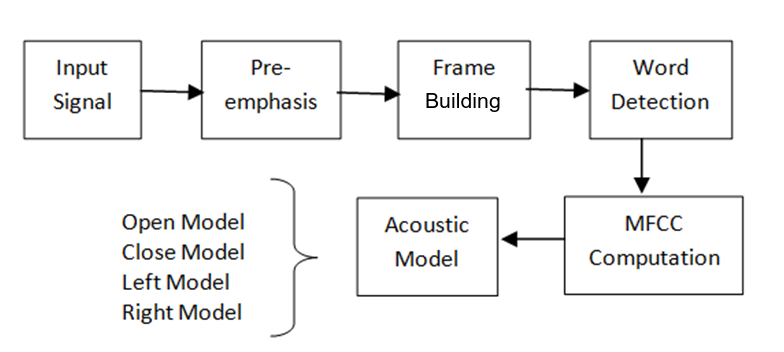
\includegraphics[width=0.6\linewidth]{figs/1bloquesTraining}
\end{center}
   \caption{Blocks for Training Stage.}
\label{trainingBlocks}
\end{figure}

Testing Stage

\begin{figure}[!ht]
\begin{center}
   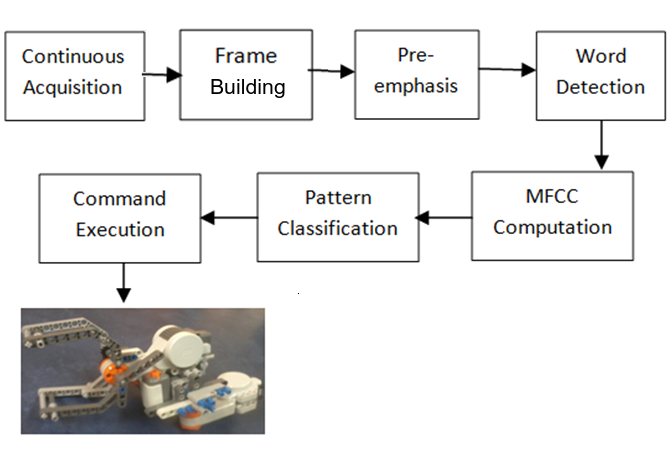
\includegraphics[width=0.6\linewidth]{figs/11bloquesTesting}
\end{center}
   \caption{Blocks for Testing Stage.}
\label{trainingBlocks}
\end{figure}
\end{block}


\end{textblock}

\begin{textblock}{39.5}(43.05,19)

\begin{block}{Results}

\begin{table}[h]
\centering
%\tiny
%\scriptsize
\footnotesize
%\small
\begin{tabular}{||p{3.5cm}||p{4cm}||p{3cm}||p{4cm}||p{4cm}||p{4cm}||p{4cm}||p{6cm}||}%p{3cm}
\hline 
\textbf{Speaker} &  \textbf{GMM Number} & \textbf{No. of words} & \multicolumn{4}{|c||}{\textbf{Command Performance (\%)}} & \textbf{Global Performance (\%)}\\
\cline{4-7}
& & & \textbf{Open} & \textbf{Close} & \textbf{Left} & \textbf{Right} & \\
\hline \hline

1 &5 &17 &94.11 &100 &94.11 &100 & \textbf{97.05} \\
\hline 
1 &8 &17 &100 &88.23 &82.35 &94.11 &\textbf{88.23} \\
\hline
1 &11 &17 &94.11 &82.35 &82.35 &94.11 &\textbf{88.23} \\
\hline
2 &5 &18 &100 &94.11 &94.11 &100 & \textbf{97.05}\\
\hline
2 &8 &16 &100 &100 &100 &100 & \textbf{100}\\
\hline
2 &11 &18 &100 &100 &100 &100 & \textbf{100}\\
\hline

\end{tabular}
\caption{Performance of the Voice Recognition System}
\label{performance}
\end{table}

\begin{table}[!ht]
	\small
	\begin{center}	
	\begin{tabular}{|c | p{17.5cm} | c|}
	\hline
	\textbf{Approach} & \textbf{Description} & \textbf{Performance} \\
	\hline
	\hline
	Tezer \cite{Tezer} &
		Used LPC and DTW. Implemented in MATLAB. &
		86\% \\
	Beritelli \cite{Beritelli} &
		Used VQ. Proposed to noise-robust application &
		~92\% \\
	Bedoya \cite{Bedoya} &
		Used wavelts, HMMs and MFCCs &
		98\% \\
	Phokharatkul \cite{Phokharatkul} &
		Used filter banks and Mel scale analysis &
		96.3\% \\
	Ali \cite{Ali} &
		Used MFCCs and ANN. Isolated or continuous speech mode &
		~96\% \\
	Chin \cite{Chin} &
		Used MFCCs and ANN&
		98.9\% \\
	Ours &
		Used MFFCs and GMMs, implemented in MATLAB &
		95.09\%\\
	\hline
	\end{tabular}
	\end{center}	
	\caption{Comparision of different speech recognition systems}
	\label{table_comp}
\end{table}

\end{block}

\begin{block}{Conclusions}
In this paper we presented an speaker-dependent speech recognition system based on Mel Frequency Cepstral Coefficients (MFCCs) for extracting features and Gaussian Mixture Models (GMMs) for creating the model of each command. We test the systems with two different speakers and the worst case was $91.17\%$ (average of global performance for speaker $1$) of accuracy for a speaker. For a particular command, the worst case was $82.35\%$ and the average of the global performance of the system was $95.09\%$ (see Results section).

As future work, we propose the evaluation of the system with more than four commands and the creation of models with utterances from different speakers in order to test the capability of the system to be speaker-independent.
\end{block}

\begin{block}{References}
\small
\bibliography{\jobname}
\end{block}

\end{textblock}

\end{frame}
\end{document}
